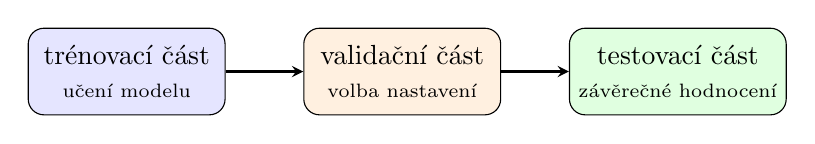
\begin{tikzpicture}[
    >=stealth,
    box/.style={
        draw,
        rounded corners=2mm,
        minimum width=25mm,
        minimum height=11mm,
        align=center
    },
    arr/.style={
        ->,
        thick,
        rounded corners=2mm
    }
]
    \node[box, fill=blue!10] (train) at (-3.5,0)
        {trénovací část\\\scriptsize učení modelu};

    \node[box, fill=orange!12] (validate) at (0,0)
        {validační část\\\scriptsize volba nastavení};

    \node[box, fill=green!12] (test) at (3.5,0)
        {testovací část\\\scriptsize závěrečné hodnocení};
    
    \draw[arr] (train) -- (validate);
    \draw[arr] (validate) -- (test);

\end{tikzpicture}
